% This LaTeX template was created for ECE431 Lab Reports at the University of Illinois @ Urbana-Champaign
% Created by Matt Magill, Spring 2012

\documentclass[11pt]{article}

% Standard packages for figures, citations, math, tables, etc.
% Feel free to add more as needed!
\usepackage{amssymb}
\usepackage{graphicx}
\usepackage{epstopdf} 
\usepackage{cite}
\usepackage[cmex10]{amsmath}
\interdisplaylinepenalty=2500 
\usepackage{mdwmath}
\usepackage{mdwtab}
\usepackage{color}
\usepackage{pgfplots}
\usepackage{multirow}
\usepackage[caption=false,font=footnotesize]{subfig}
\usepackage{verbatim}
\usepackage{appendix}
\usepackage{booktabs}

% Packages for formatting with 1 in margins and doublespacing
\usepackage[latin1]{inputenc}
\usepackage[left=1in,top=1in,right=1in,bottom=1in,nohead]{geometry}
\usepackage{setspace}
\doublespacing

% Define the location of your figures in order to avoid writing absolute file location
\graphicspath{{figures/}}	

% It is often convenient to create new commands for commonly used items
\renewcommand{\div}[1]{\nabla \cdot #1} % divergenge of a vector (\div)
\newcommand{\curl}[1]{\nabla \times #1} % curl of a vector (\curl)


%% This can be used to indent paras (if you ever need it) - SSG
\newenvironment{myindentpar}[1]%
 {\begin{list}{}%
         {\setlength{\leftmargin}{#1}}%
         \item[]%
 }
 {\end{list}}

\begin{document}

% Title Page
\begin{titlepage}
\begin{center}
{\LARGE \textsc{ECE 395 Advanced Digital Projects Lab} \\ \vspace{8pt}}
{\Large \textsc{Optical Guitar} \\ \vspace{8pt}} 
\rule[13pt]{\textwidth}{1pt} \\ \vspace{150pt}
{\Large \textsc{Final Report - Fall 2012 } \\ \vspace{8pt}}

{\large Sartaj S. Grewal\\ \vspace{1pt}
\large grewal2@illinois.edu\\ \vspace{16pt}
 \today}
\vfill
\end{center}
%\begin{flushright} 
%{\large
%{\bf Leader:} Leader's name\\
%{\bf Recorder:} Recorder's name}
%\end{flushright}

\pagenumbering{Roman}	% Page count done in roman numerals
\end{titlepage}
\setcounter{page}{2}

\newpage{}

\tableofcontents

\newpage{}


% Introduction
\section{Overview}

{The objective of the project is to replace the strings of a traditional guitar with lasers. Most of the existing laser guitars include supplementary sensors but in this project lasers are the only sensing mechanism used. The implementation of the project can be broadly classified on the area of the guitar, namely the fretboard and the picking area. Implementation for the pricking area require a simple setup of a laser and a photodiode with operation requiring hindering the path of the laser rays. This work has been deferred for next semester and this semester most of the work was done on the implementation on the fretboard part. It can be broken down into three broad areas of work, namely,  constructing the laser array, building the sensor framework and synthesizing the output of the sensor framework. }

\textbf{Please note that the references, the code repository and the parts list have been provided in the appendix.}


\section{Design}

The project involved arduous design review because using an optimal configuration  would reduce the specifications requirements for many components and the error induced in the system. In this section, many of the designs, the choices and the requirements have been discussed.

\subsection{Laser Array}

The laser array was designed to be close to the surface of the guitar parallel to the line of path of the strings. It was done so that lasers rays would not be blocked by the other fingers of the playing hand in error. 

For this project, the laser diodes VLM-650001 LPT and VLM-650001 LPA from Digikey have been used. The reason for using visible laser diodes was because it was desired to be able to see the laser rays and hence visible lasers; they were also readily available, moderately priced and safe to use.  The laser diodes include a Automatic Power Control(APC) circuit, which when used in conjunction of voltage regulators, helps control the laser output to steady level.

\begin{figure}[!h]
\centering
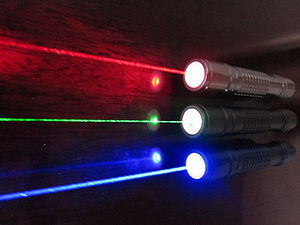
\includegraphics[width=0.5\textwidth]{lasers.jpg}
\caption{Lasers (Courtesy:Wikipedia.org)}
\label{lasers}
\end{figure}

\newpage{}

\subsection{Sensors}

One of the fundamental problems within the project is the determination of the note being played on the fretboard. Three possible design configurations were discussed to solve this problem and the laser distance detection technique was chosen to be best suited for the application.

\subsubsection{Camera Triangulation}

A popular technique used in distance estimation and triangulation is to use two or more cameras pointed at the object, in this case that would be the fretboard. The distance is estimated based on the angle of the cameras and the projected distance obtained in the image. The benefits of this technique are that high speeds of propagation of light do not affect the outcome and help reduce the system requirements greatly. 

Although camera triangulation is a great technique that offers easier to use implementation, in the case of this project it would not function optimally. The camera angle required to make the device rid of blocking due to the hand or other fingers would too large and would sacrifice the prudence of the implementation. 


\newpage{}

\begin{figure}[!h]
\centering
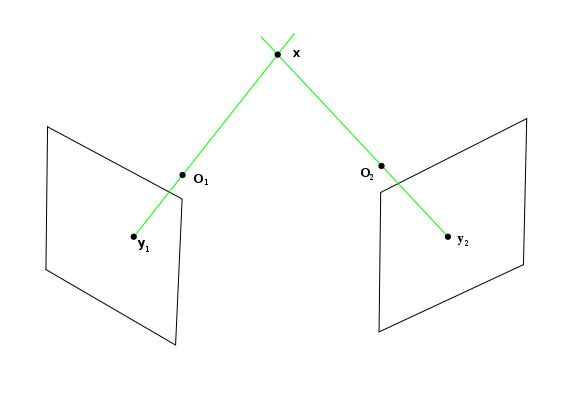
\includegraphics[width=0.5\textwidth]{camera.png}
\caption{Camera Triangulation (Courtesy: Wikipedia.org)}
\label{camera}
\end{figure}

\subsubsection{Distributed Sensors}

Another idea that was discussed regarding having sensors on the pick used to the play the guitar and also on the fingers of the playing hand. The sensors would be used to detect laser and provide feedback to the user and the guitar. It implemented correctly, this idea serves the benefit that the operation of the final device would be essentially error proof. But the problems associated with this configuration including manufacture of custom miniature sensors, magnitude of sensors required and orientations make it impractical. 

\begin{figure}[!h]
\centering
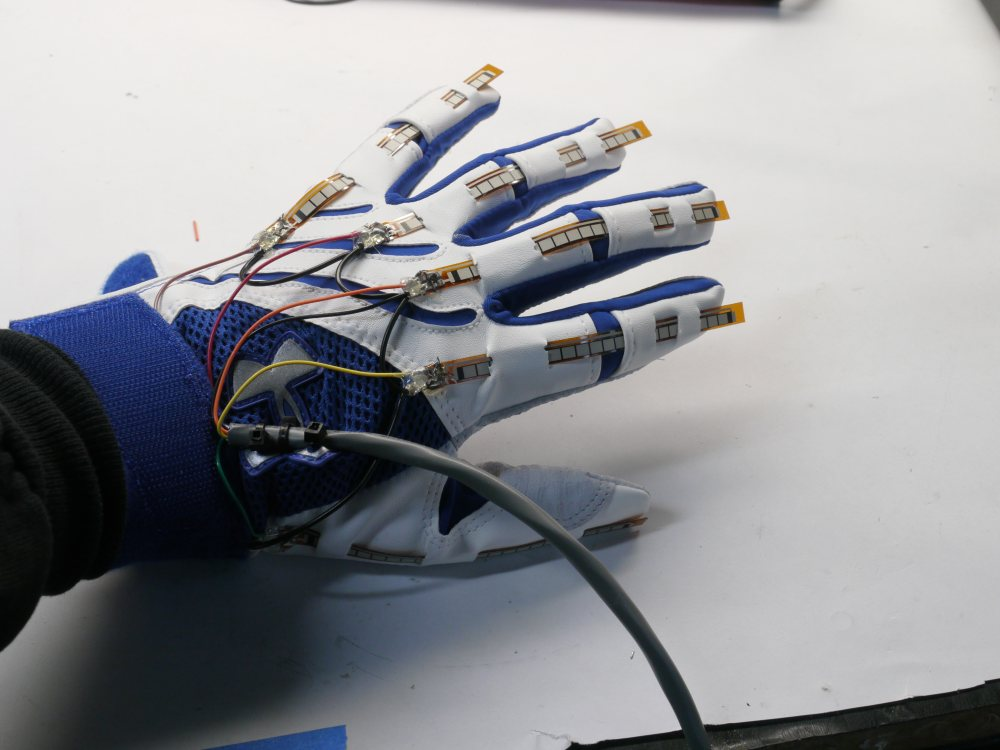
\includegraphics[width=0.5\textwidth]{glove.jpg}
\caption{Sensor Glove(Courtesy: http://benkrasnow.blogspot.com/2010/12/diy-10-finger-flex-sensor-gloves-for.html)}
\label{glove}
\end{figure}


\subsubsection{LIDAR Implementation}

Laser Distance Detection is the technique being used in the project. This technique includes firing the laser at the object in pulses and the time taken of the reflection is recorded, and used to measure the distance. One of the cons for this implementation is the inclusion of speed of light into the design considerations and makes the design very complex. High speed op-amps and comparators have to be used to get a viable measurement and not suffer from huge delays. 

Although this technique is one of the toughest to implement, the exact use of the device would not be to measure the exact distance of the finger from the laser array bridge, but the relative distance between different frets. For the same reason, high precision is required and that is why the ACAM TDC GP21 chip is used in the project. The chip is simply a high speed counter (resolution in pico seconds) with many additional features, including SPI communication. 

\begin{figure}[!h]
\centering
\includegraphics[width=0.5\textwidth]{lidar.jpg}
\caption{Handheld LIDAR (Courtesy: http://www.stalkerradar.com/oem/Lidar-RR.html)}
\label{lidar}
\end{figure}

\newpage{}

\section{Implementation}

In this section, all the progress for the semester has been detailed. The work was mostly done in designing the laser detection module and doing basic initialization code for the the Renesas micro controller. 

\subsection{Laser Distance Detection Module}

Much of the design discussed here has been derived from the thesis of the student group of UCF (reference in Appendix). The overview of the design is provided in the Fig.~\ref{overview}, which shows a basic LIDAR application design.

\begin{figure}[!h]
\centering
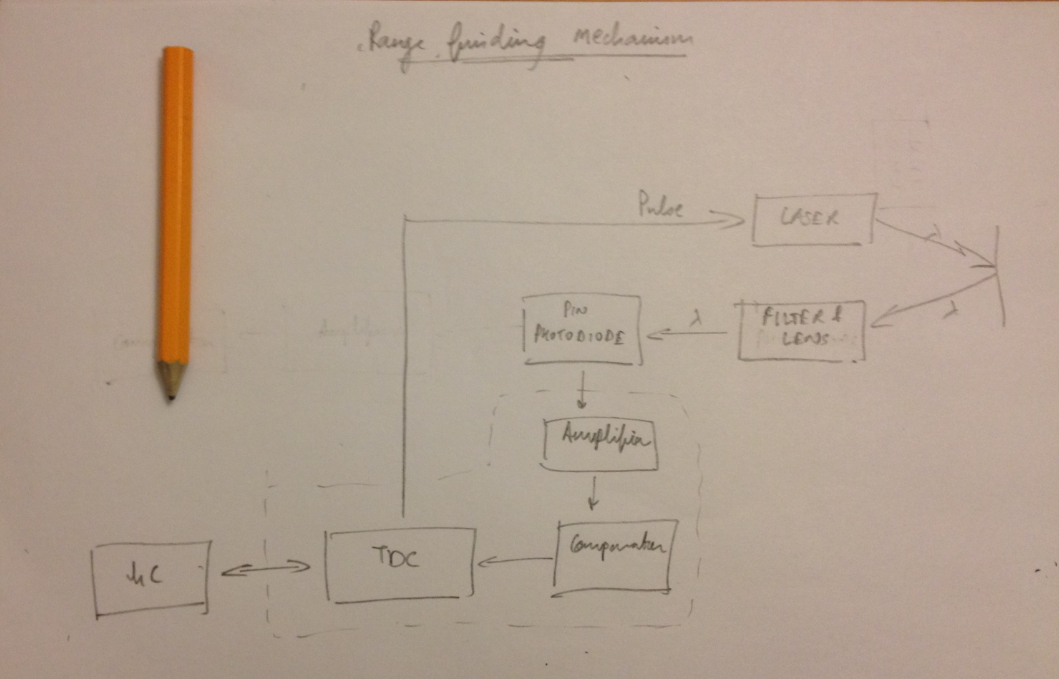
\includegraphics[width=0.8\textwidth]{overview.png}
\caption{Overview of the Design}
\label{overview}
\end{figure}

The laser diodes have been discussed in the previous sections. In the subsequent sub sections, each of the blocks and the design choices associated will be discussed individually.

\subsubsection{Filter and Lens}
















 




\end{document}